\documentclass[11pt,a4paper]{article}
\usepackage[utf8]{inputenc}
\usepackage[T1]{fontenc}
\usepackage[spanish,es-noshorthands]{babel}
\usepackage[margin=2.1cm]{geometry}
\usepackage{amsmath,amssymb}
\usepackage{graphicx}
\usepackage{booktabs}
\usepackage{xcolor}
\usepackage[colorlinks=true,linkcolor=blue!50!black,urlcolor=blue!50!black]{hyperref}
\setlength{\parskip}{4pt}
\setlength{\parindent}{0pt}
\newcommand{\dd}{\mathrm{d}}
\title{Diagramas de cuerpo libre del Segway con patas\\
\large Pata parada en la postura más desfavorable, y péndulo invertido sobre ruedas}
\author{Proyecto Segway con patas -- Robótica II, UNCUYO}
\date{\today}

\begin{document}
\maketitle

Dos configuraciones: la pata con la cabina fija, cargada con el peso del robot, que es la que dimensiona el
servo; y el robot entero como péndulo invertido sobre las ruedas, que es la que gobierna el equilibrio. De la
primera sale el par del servo por equilibrio estático, calculado a mano y comparado con el resultado de
Lagrange de \texttt{dinamica\_resumen.pdf}. De la segunda salen las ecuaciones de Newton--Euler que el
modelo de la planta tiene que reproducir.

\section{Pata parada, \(\theta=10^\circ\)}

\begin{center}
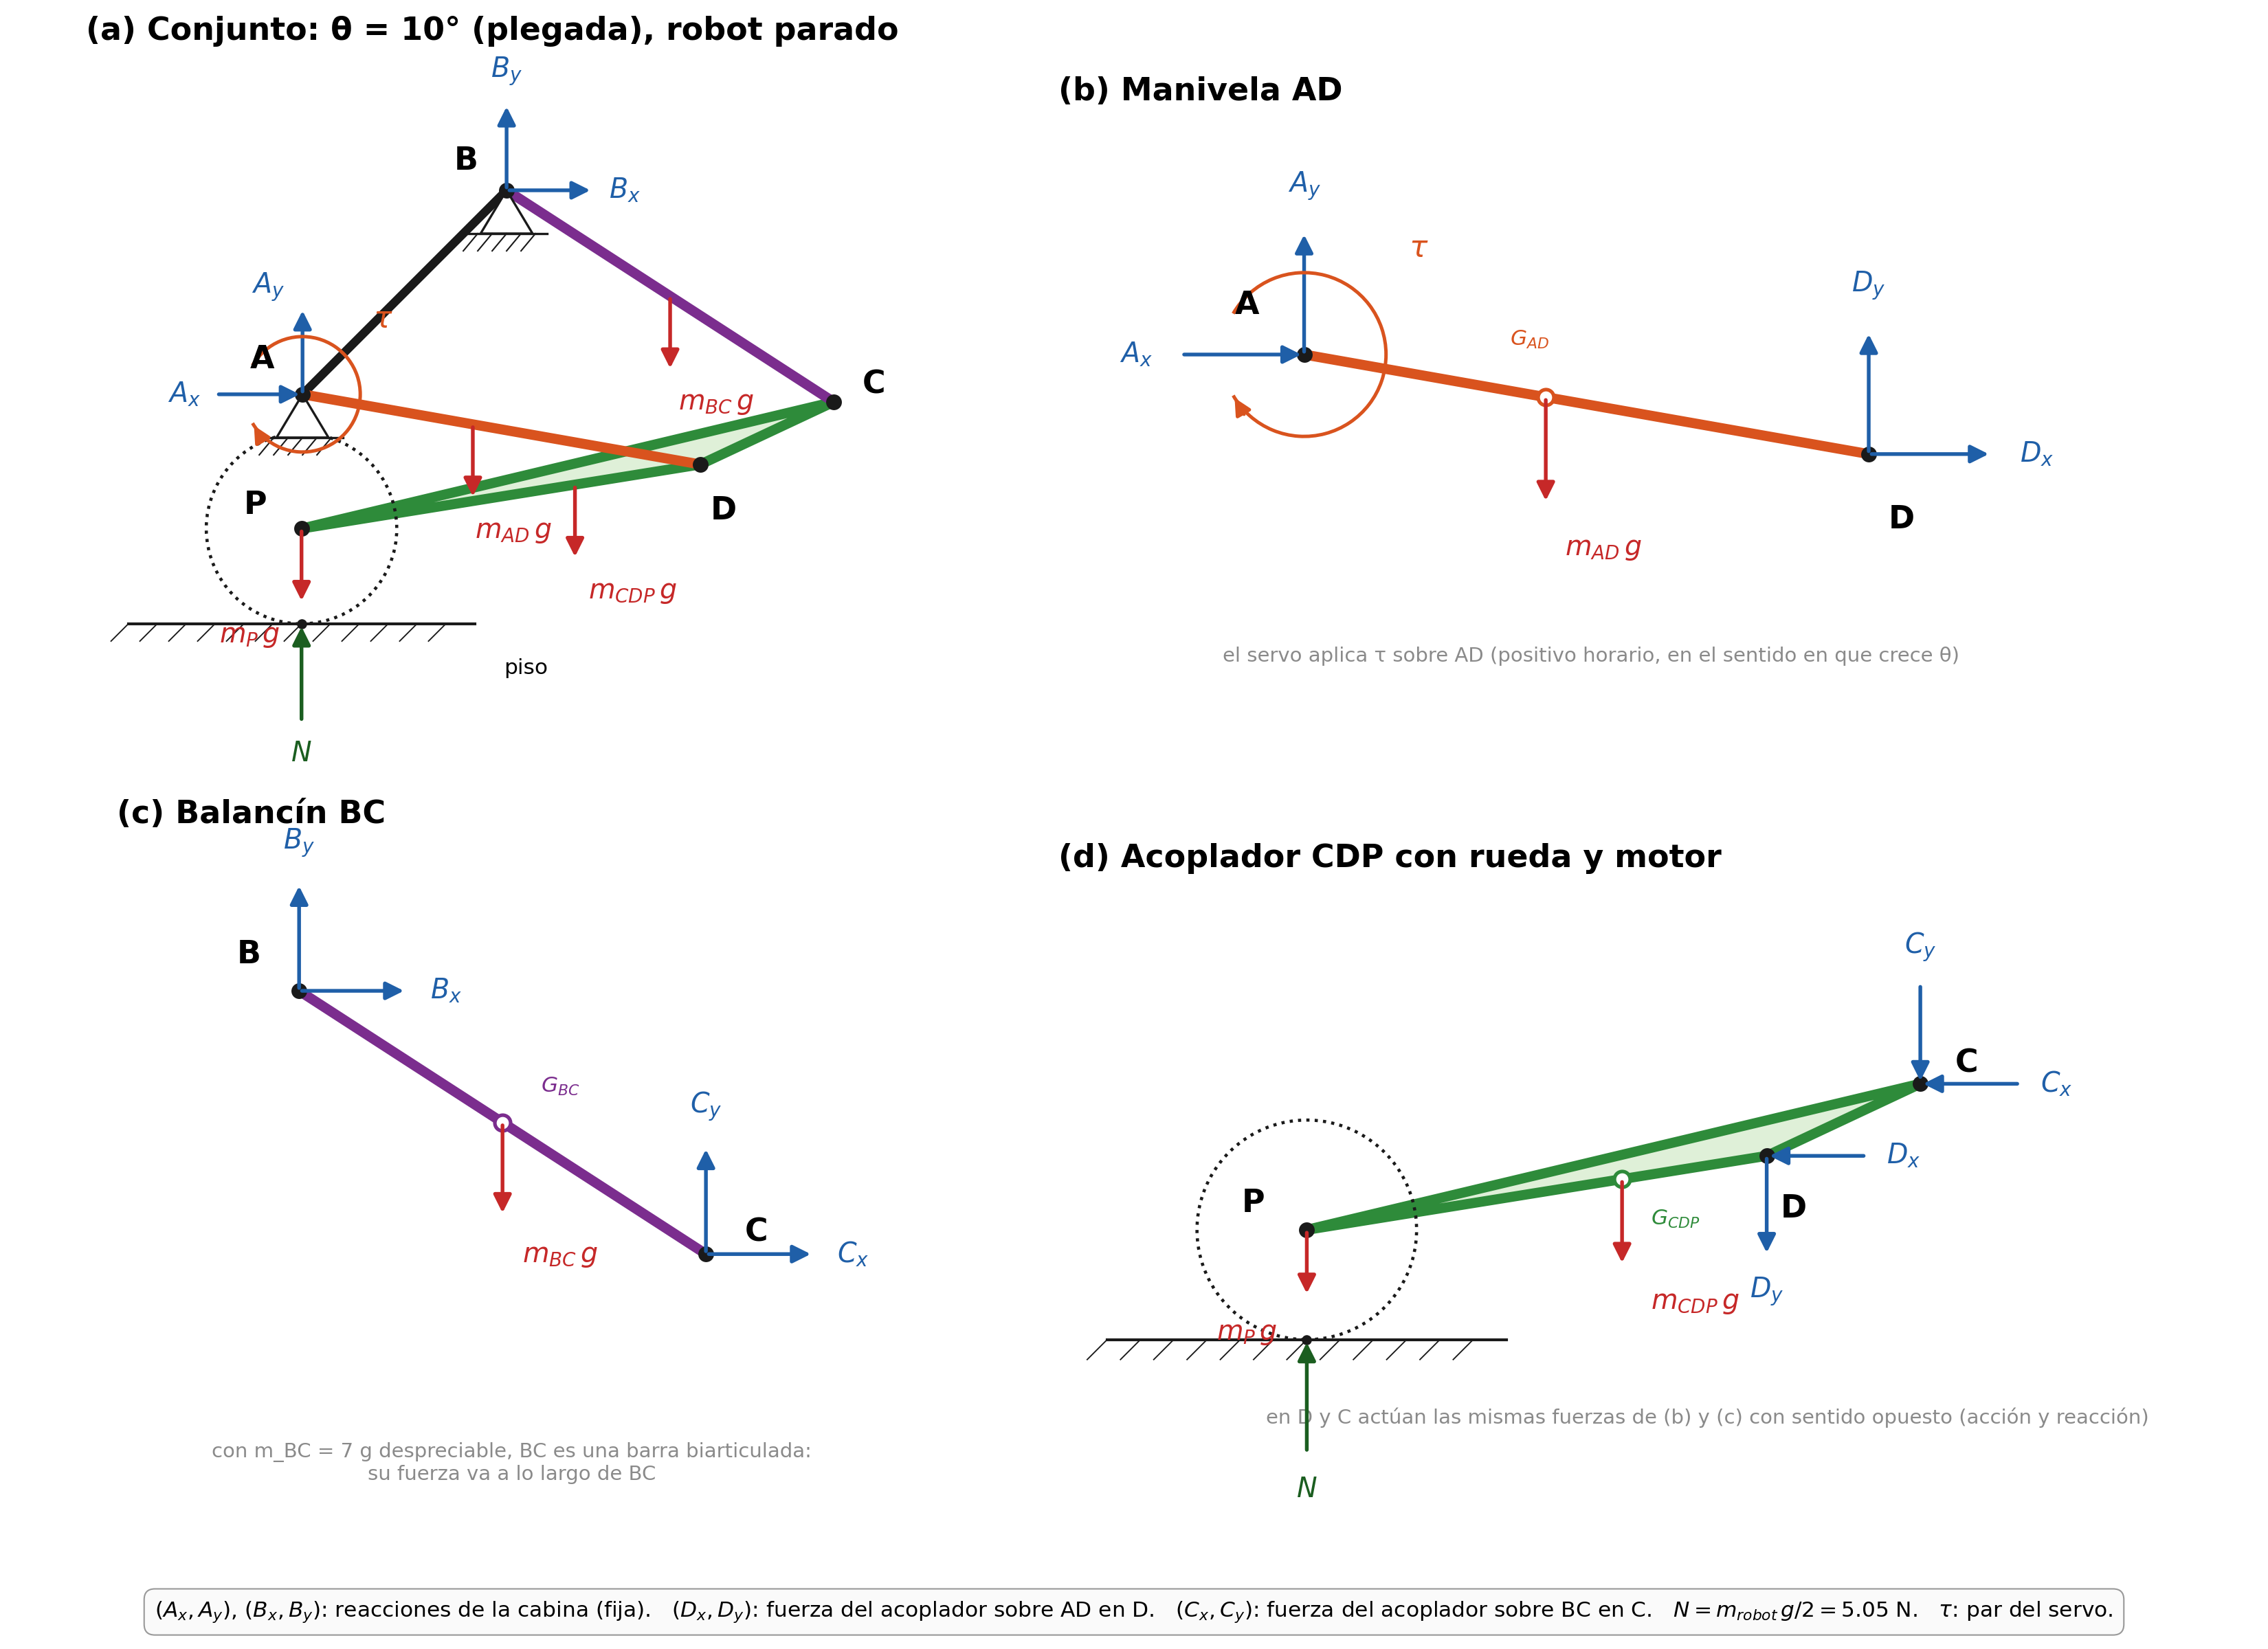
\includegraphics[width=\textwidth]{dcl_pata.png}
\end{center}

\textbf{Configuración.} Cabina fija (pivotes \(A\) y \(B\)), pata plegada (\(\theta=10^\circ\)), robot parado
sobre las dos ruedas: la reacción del piso por pata es \(N=m_{robot}\,g/2=5.05\) N, vertical, sin fuerza
horizontal. Es la postura en la que el servo pide más par, porque el brazo \(|y_P'|\) es máximo. Tres
cuerpos: manivela \(AD\), balancín \(BC\), y el acoplador \(CDP\) con la rueda y el motor colgados de \(P\).

\textbf{Convención.} \((A_x,A_y)\) y \((B_x,B_y)\) son las reacciones de la cabina; \((D_x,D_y)\) es la fuerza
del acoplador sobre \(AD\) en \(D\), y \((C_x,C_y)\) la del acoplador sobre \(BC\) en \(C\); sobre el
acoplador actúan con signo opuesto. \(\tau\) es el par del servo, positivo horario (en el sentido en que crece
\(\theta\)); en las ecuaciones de momentos, antihorario positivo, entra como \(-\tau\). Ejes con origen en
\(A\), \(y\) hacia arriba. Posiciones en \(\theta=10^\circ\) (de la cinemática), en mm:
\[
B=(70.7,\;70.7),\quad C=(184.0,\;-2.6),\quad D=(137.9,\;-24.3),\quad P=(-0.3,\;-46.5),
\]
\[
G_{AD}=(59.0,\;-10.4),\quad G_{BC}=(127.4,\;34.0),\quad G_{CDP}=(94.4,\;-31.3).
\]
Pesos: \(m_{AD}g=0.285\) N, \(m_{BC}g=0.069\) N, \(m_{CDP}g=0.191\) N, \(m_Pg=1.226\) N.

\textbf{Ecuaciones de equilibrio.} Suma de fuerzas y de momentos en cada cuerpo (momentos respecto del pivote
de cada barra y respecto de \(D\) en el acoplador; el momento de una fuerza \((F_x,F_y)\) aplicada en
\(\mathbf{r}\) es \(r_xF_y-r_yF_x\)):
\begin{align}
AD:&\quad A_x+D_x=0,\qquad A_y+D_y-m_{AD}g=0,\qquad -\tau+x_D D_y-y_D D_x-m_{AD}g\,x_{G_{AD}}=0. \label{eq:AD}\\
BC:&\quad B_x+C_x=0,\qquad B_y+C_y-m_{BC}g=0, \notag\\
   &\quad (x_C-x_B)\,C_y-(y_C-y_B)\,C_x-m_{BC}g\,(x_{G_{BC}}-x_B)=0. \label{eq:BC}\\
CDP:&\quad -D_x-C_x=0,\qquad -D_y-C_y-(m_{CDP}+m_P)\,g+N=0, \notag\\
   &\quad -(x_C-x_D)\,C_y+(y_C-y_D)\,C_x-m_{CDP}g\,(x_{G_{CDP}}-x_D)-(m_Pg-N)\,(x_P-x_D)=0. \label{eq:CDP}
\end{align}
Nueve ecuaciones lineales con nueve incógnitas, \(A_x,A_y,\tau,B_x,B_y,C_x,C_y,D_x,D_y\). Resueltas en la
sección 4 de \texttt{dinamica\_pata.m}:

\begin{center}\small
\begin{tabular}{lrrrrrrrrr}
\toprule
 & \(A_x\) & \(A_y\) & \(B_x\) & \(B_y\) & \(C_x\) & \(C_y\) & \(D_x\) & \(D_y\) & \(\tau\) \\
\midrule
valor & 10.13 N & \(-9.87\) N & \(-10.13\) N & 6.59 N & 10.13 N & \(-6.52\) N & \(-10.13\) N & 10.16 N & 1.137 N\,m \\
\bottomrule
\end{tabular}
\end{center}

\(\tau=1.137\) N\,m \(=11.6\) kg\,cm, igual al \(\tau_{est}=V'-N\,y_P'\) de Lagrange hasta el redondeo de
máquina (\(10^{-15}\)): las dos formas de plantear la estática coinciden. La fuerza en \(BC\) vale 12.0 N y
va a lo largo de la barra (tracción); \(A_x+B_x=0\) porque no hay fuerza horizontal externa.

\textbf{Cálculo a mano en tres pasos.} Despreciando el peso del balancín (7 g), \(BC\) es una barra
biarticulada y su fuerza va a lo largo de \(BC\): \((C_x,C_y)=s\,\mathbf{u}\), con
\(\mathbf{u}=(C-B)/|C-B|=(0.840,\,-0.543)\).
\begin{enumerate}
\item Momentos en \(D\) sobre el acoplador, ecuación \eqref{eq:CDP}, con \(C_x=s\,u_x\), \(C_y=s\,u_y\):
\begin{gather*}
s=\frac{N\,(x_P-x_D)-m_{CDP}g\,(x_{G_{CDP}}-x_D)-m_Pg\,(x_P-x_D)}{(x_C-x_D)\,u_y-(y_C-y_D)\,u_x}\\
 =\frac{5.05\,(-0.1382)-0.191\,(-0.0435)-1.226\,(-0.1382)}{-0.0433}=\frac{-0.520}{-0.0433}=12.0\ \text{N}.
\end{gather*}
\item Suma de fuerzas en el acoplador: \(D_x=-s\,u_x=-10.1\) N,
\(D_y=N-(m_{CDP}+m_P)\,g-s\,u_y=5.05-1.418+6.54=10.17\) N.
\item Momentos en \(A\) sobre \(AD\), ecuación \eqref{eq:AD}:
\(\tau=x_D D_y-y_D D_x-m_{AD}g\,x_{G_{AD}}=0.1379\cdot10.17-0.0243\cdot10.10-0.285\cdot0.059=1.140\) N\,m.
\end{enumerate}
Diferencia con el valor exacto: 0.2 por ciento, que es el peso del balancín despreciado. Con el servo de
21 kg\,cm el margen en esta postura es 1.8.

\section{Péndulo invertido sobre ruedas}

\begin{center}
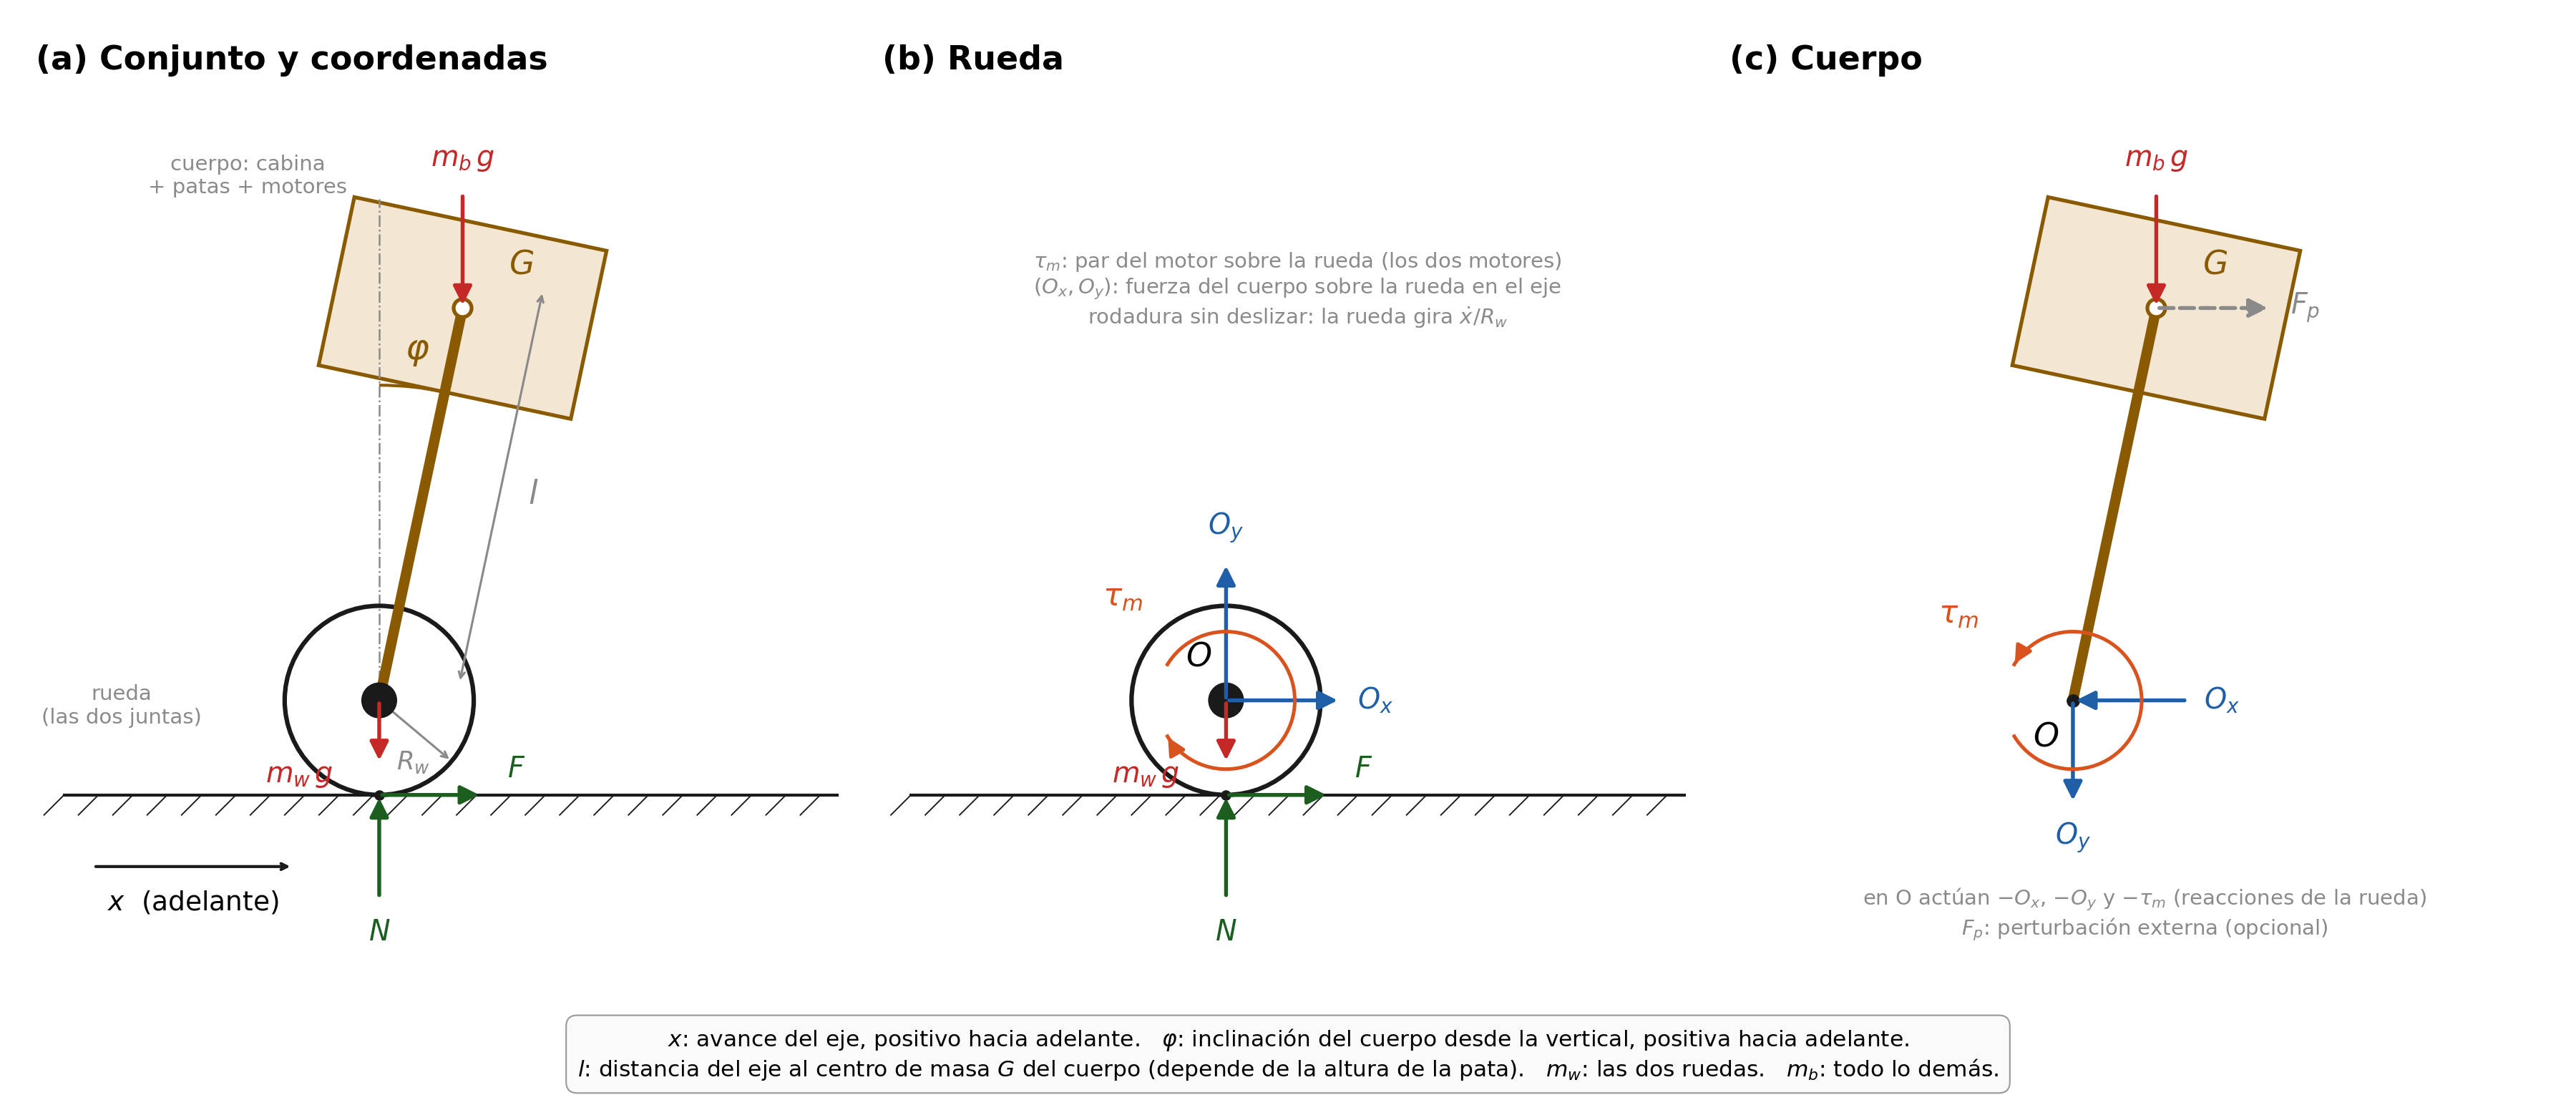
\includegraphics[width=\textwidth]{dcl_segway.png}
\end{center}

\textbf{Configuración.} Plano sagital, piso horizontal, pata fija (una altura dada). Dos cuerpos: la rueda
(las dos juntas: masa \(m_w\), inercia \(J_w\), radio \(R_w\)) y el cuerpo (cabina, patas y motores: masa
\(m_b\), inercia \(J_b\) respecto de su centro de masa \(G\), a distancia \(l\) del eje). Coordenadas:
\(x\) avance del eje, positivo hacia adelante; \(\varphi\) inclinación del cuerpo desde la vertical, positiva
hacia adelante. Rodadura sin deslizar: la rueda gira \(\dot x/R_w\). El motor aplica \(\tau_m\) sobre la
rueda (los dos juntos) y \(-\tau_m\) sobre el cuerpo. \((O_x,O_y)\) es la fuerza del cuerpo sobre la rueda en
el eje. Vista desde el lado derecho del robot: aquí el frente queda a la derecha (en las figuras de la pata
queda a la izquierda).

\textbf{Newton--Euler de cada cuerpo.} Momentos positivos en el sentido de \(\varphi\) (horario en la
figura). Centro de masa del cuerpo: \(x_G=x+l\sin\varphi\), \(y_G=R_w+l\cos\varphi\).
\begin{align}
\text{rueda:}&\quad m_w\ddot x=F+O_x,\qquad 0=N-m_wg+O_y,\qquad J_w\frac{\ddot x}{R_w}=\tau_m-F\,R_w, \label{eq:rueda}\\
\text{cuerpo:}&\quad m_b\ddot x_G=-O_x+F_p,\qquad m_b\ddot y_G=-O_y-m_bg, \notag\\
&\quad J_b\ddot\varphi=-\tau_m+l\cos\varphi\,O_x-l\sin\varphi\,O_y+h_pF_p. \label{eq:cuerpo}
\end{align}
(\(F_p\) es una perturbación horizontal aplicada a altura \(h_p\) sobre \(G\); se deja en cero salvo en los
escenarios de empujón.)

\textbf{Ecuaciones de movimiento.} Con \(\ddot x_G=\ddot x+l\cos\varphi\,\ddot\varphi-l\sin\varphi\,\dot\varphi^2\)
y \(\ddot y_G=-l\sin\varphi\,\ddot\varphi-l\cos\varphi\,\dot\varphi^2\), se despejan \(O_x\), \(O_y\) y \(F\)
de \eqref{eq:rueda}--\eqref{eq:cuerpo} y quedan dos ecuaciones en \(x\) y \(\varphi\) (con \(F_p=0\)):
\begin{equation}
\boxed{\;
\begin{aligned}
\Bigl(m_b+m_w+\frac{J_w}{R_w^2}\Bigr)\ddot x+m_b\,l\cos\varphi\,\ddot\varphi-m_b\,l\sin\varphi\,\dot\varphi^2&=\frac{\tau_m}{R_w},\\
\bigl(J_b+m_b\,l^2\bigr)\ddot\varphi+m_b\,l\cos\varphi\,\ddot x-m_b\,g\,l\sin\varphi&=-\tau_m .
\end{aligned}
\;}
\label{eq:segway}
\end{equation}
La normal, que sirve para saber si la rueda sigue apoyada, es
\(N=(m_b+m_w)\,g-m_b\,l\,(\sin\varphi\,\ddot\varphi+\cos\varphi\,\dot\varphi^2)\).

Dos lecturas inmediatas. Sostener el cuerpo inclinado \(\varphi_0\) con las ruedas trabadas pide
\(\tau_m=m_b\,g\,l\sin\varphi_0\): con \(m_b\approx0.97\) kg y \(l\approx0.14\) m, 0.19 N\,m para \(8^\circ\),
repartido entre los dos motores. Y sin par (\(\tau_m=0\)) el cuerpo se cae: linealizando la segunda ecuación
queda \(\ddot\varphi\approx m_b\,g\,l\,\varphi/(J_b+m_b l^2)\), que crece como una exponencial. El modelo de
la planta (\texttt{planta/}) deduce \eqref{eq:segway} por Lagrange y tiene que coincidir con esto término a
término; después agrega \(\theta\) como tercera coordenada, y \(l\) pasa a depender de \(y_P(\theta)\).

\section{Archivos}

\begin{itemize}
\item \texttt{dcl\_pata.py} \(\to\) \texttt{dcl\_pata.png}: el diagrama de la sección 1, en \(\theta=10^\circ\)
  (cambiar \texttt{THETA} para otra postura).
\item \texttt{dcl\_segway.py} \(\to\) \texttt{dcl\_segway.png}: el diagrama de la sección 2.
\item \texttt{../dinamica/dinamica\_pata.m}, sección 4: resuelve las nueve ecuaciones de la sección 1, las
  compara con Lagrange y hace el cálculo a mano de tres pasos.
\end{itemize}

\end{document}
